\chapter{Physical description of the climate system}\label{ch:climate-system-description}
\lastupdated{2024-12-02 23.47}{\chapterOneIntro}

\section{Atmosphere}\label{sec:atm-description}

\subsection{Atmospheric composition}\label{subsec:atm-composition]}

The atmosphere is a gaseous envelope that surrounds the Earth, acting as a protective envelope essential for life.
It is composed of a mechanical mixture of several gases, with \emph{nitrogen} (\ce{N2}) being the most abundant (\qty{78}{\percent} of the volume of dry air),
followed by \emph{oxygen} (\ce{O2}) \qty{20.95}{\percent}, \emph{argon} (\ce{Ar}) \qty{0.93}{\percent},
and \emph{carbon dioxide} \ce{CO2} \qty{0.037}{\percent}.
Trace gases like \emph{Neon} (\ce{Ne}), \emph{helium} (\ce{He}), \emph{methane} (\ce{CH4}), and hydrogen (\ce{H}) also contribute to its composition, along
with varying amounts of water vapor, which depend on factors such as location, evaporation rates, and temperature.

This gaseous mixture is held to the Earth by gravity, which causes the atmosphere to exert a pressure. Near the surface, the pressure is greatest, approximately \qty{1.013e3}{\milli\bar} at sea level, and it decreases with altitude. This reduction in pressure reflects the compressibility of gases, making the atmosphere densest near the ground. This characteristic distinguishes the atmosphere from the ocean, where the density remains relatively uniform due to the near incompressibility of liquids.

\subsection{The Vertical Temperature Profile}

The atmosphere exhibits a distinct temperature profile that changes with altitude and varies depending on the region and season. These variations define the layers of the atmosphere, each with unique characteristics and processes.

\begin{itemize}
	\item \textbf{The Troposphere}: is the lowest layer, extending from the surface up to about 17 kilometers in the tropics and
	      \qtyrange{8}{9}{\kilo\meter} in polar regions.
	\item In this layer, the temperature generally decreases with altitude at an average rate of \qty{6.4}{\celsius.\kilo\meter^{-1}}. This gradient arises because the surface absorbs heat from the sun and transfers it to the air above, while higher altitudes are farther from this heat source. The troposphere is also the region where most weather phenomena, including clouds and storms, occur, making it the most dynamic part of the atmosphere.

	      At the upper boundary of the troposphere, known as the \textbf{tropopause}, the temperature reaches its minimum and remains constant for a short distance. In tropical regions, the tropopause is particularly cold, with temperatures dropping to about 190~K, marking one of the coldest points in the Earth's atmosphere.

	\item \textbf{The Stratosphere}: Above the tropopause lies the stratosphere, a more stable layer where temperatures either remain constant or begin to rise with altitude. This increase is primarily due to the absorption of ultraviolet radiation by ozone molecules, which warms this part of the atmosphere. Unlike the troposphere, the stratosphere lacks the turbulence and weather systems associated with surface heating.

	\item \textbf{The Thermosphere}: the temperature continues to increase steadily with altitude. This layer is less influenced by surface-level processes and is instead heated by the absorption of high-energy solar radiation, making it the hottest layer of the atmosphere.
\end{itemize}


\begin{table}[h!]
	\centering
	\renewcommand{\arraystretch}{1.3} % Increase row spacing
	\setlength{\tabcolsep}{4pt} % Adjust column spacing
	\begin{tabularx}{\textwidth}{@{}lXlX@{}}
		\toprule
		\textbf{}                          & \textbf{Troposphere (sum/win)}          & \textbf{Tropopause}                                                                                & \textbf{Stratosphere}       \\
		\midrule
		\textcolor{teal}{\textbf{poles}}   & \qty{280}{\kelvin} / \qty{235}{\kelvin} & \qty{9}{\kilo\meter}: \qty{230}{\kelvin} / inversion (\qty{1.5}{\kilo\meter}/\qty{2}{\kilo\meter}) & Slow Warming / Slow Cooling \\
		\textcolor{teal}{\textbf{midlat}}  & \qty{290}{\kelvin} / \qty{280}{\kelvin} & \qty{10}{\kilo\meter}: \qty{220}{\kelvin}                                                          & Slow Warming / Slow Cooling \\
		\textcolor{teal}{\textbf{tropics}} & \qty{300}{\kelvin}                      & \qty{17}{\kilo\meter}: \qty{190}{\kelvin}                                                          & Warming                     \\
		\bottomrule
	\end{tabularx}
	\caption{Temperature characteristics (expressed in \unit{\kelvin}) in different atmospheric layers.}
	\label{tab:atm-temps-layer-latitude}
\end{table}

\begin{figure}
	\centering
	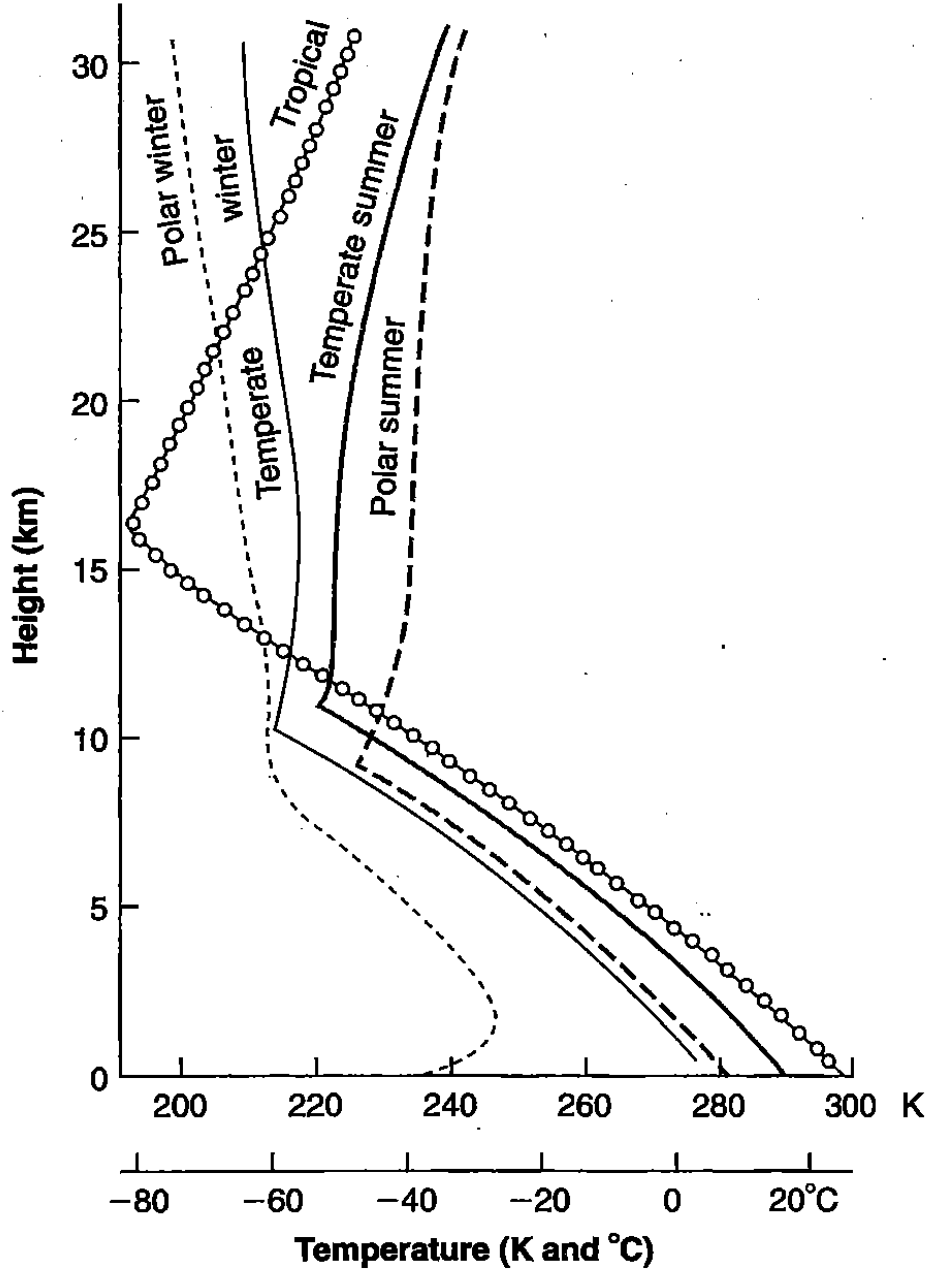
\includegraphics[width = .5 \textwidth]{figs/temp-profile-dobson}
	\caption{Atmospheric temperature profiles for different regions and season. Climatological average from~\citet{Dobson1968}.}\label{fig:temp-profile-dobson}
\end{figure}

\subsection{Regional and Seasonal Variations}

As one can grasp from~\fig{\ref{fig:temp-profile-dobson}} and from~\tabref{\ref{tab:atm-temps-layer-latitude}}, temperature profiles in the atmosphere are not uniform and vary significantly between regions and seasons.

\begin{itemize}
	\item \textbf{Polar regions:} In summer, temperatures near the surface reach about 280~K, decreasing gradually with height. In winter, surface temperatures can plummet to 235~K, but a slight increase often occurs at altitudes of \qty{1.5}{2}{\kilo\meter} due to a phenomenon called \emph{temperature inversion}. This inversion, caused by the cooling of surface air, reverses the usual trend of decreasing temperature with height.
	\item \textbf{Tropical regions:} Surface temperatures remain relatively constant, averaging around 300~K. However, as altitude increases, the temperature drops sharply, reaching the coldest point at the tropopause (about 190~K).
	\item \textbf{Mid-latitudes:} The temperature pro\file combines characteristics of both polar and tropical regions, varying more noticeably between seasons.
\end{itemize}


\subsubsection*{The Role of Energy Processes}

The vertical temperature gradient in the atmosphere is maintained by complex energy processes, including the absorption and radiation of heat, convection, and interactions with the Earth's surface. These processes vary with latitude and season, creating the dynamic and layered structure of the atmosphere.

Inversions, which occur when surface air cools significantly, disrupt the usual temperature gradient, particularly in the troposphere. These events highlight the intricate balance of energy transfer within the atmosphere and its impact on weather and climate.

\subsection{Energy balances}\label{subsec:energy-balances}
All the energy that enters the Earth’s climate system comes from the sun.
A portion of this solar energy is absorbed in the Earth's climate system and must be balanced with
outgoing energy to maintain the observed overall equilibrium state of the climate.
Such outgoing energy is emitted by the Earth's surface, the oceans, the atmosphere, the ice, and all of its life forms.

\begin{figure}
	\centering
	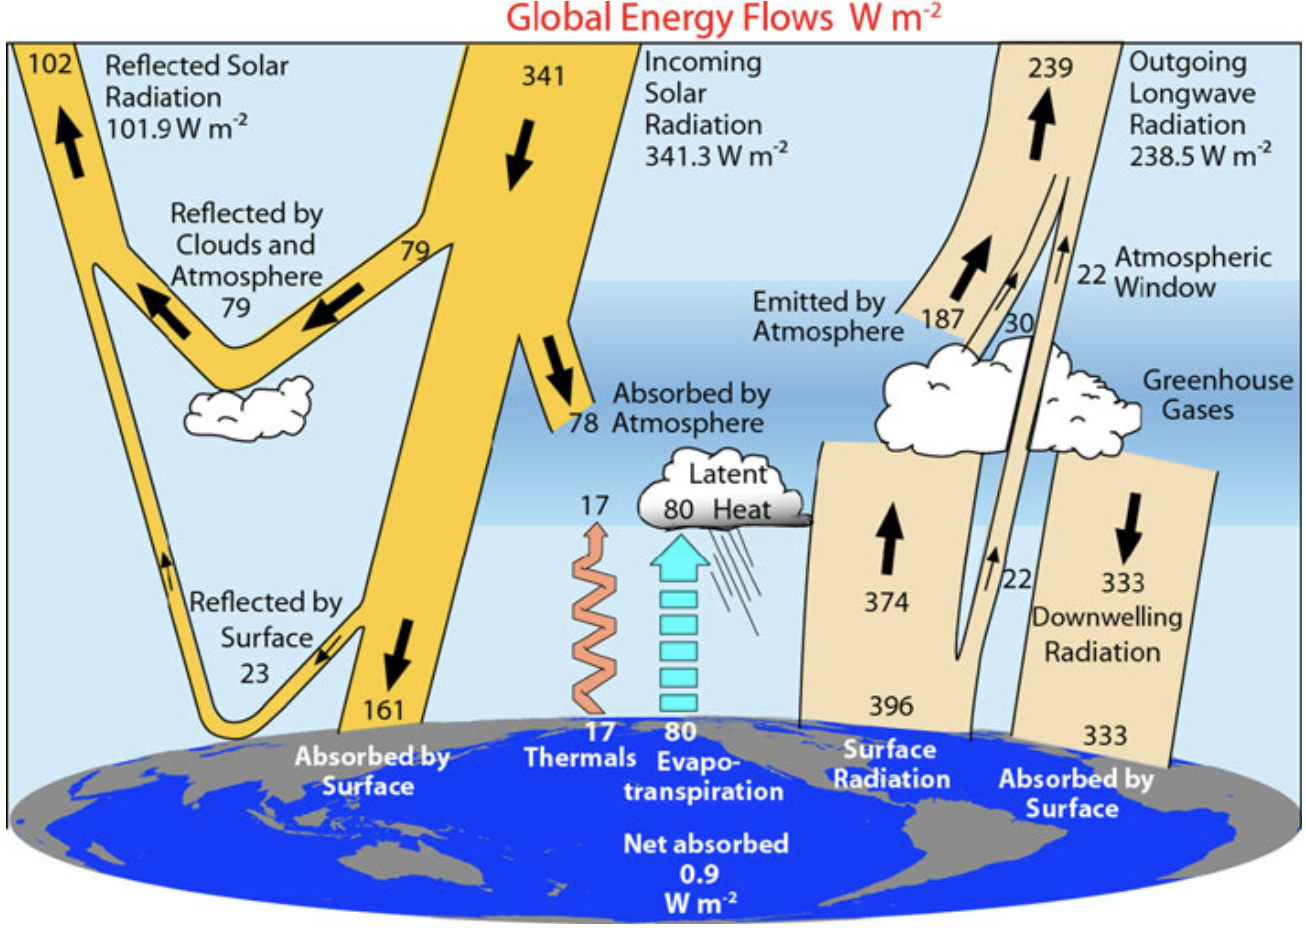
\includegraphics[width = .7 \textwidth]{figs/global-mean-energy-budget-trenberth}
	\caption{The mean global annual Earth’s energy budget for \qtyranged{2000}{2005}{} (\unit{\watt.\meter^{-2}}). The broad arrows indicate
		the schematic flow of energy in proportion to their importance. \\ Taken from~\citet{Trenberth2012}.}
	\label{fig:global-mean-energy-budget}
\end{figure}

The Earth’s climate system is driven by a balance between incoming solar radiation and outgoing terrestrial radiation, as illustrated in Figure~\ref{fig:global-mean-energy-budget}. Of the \qty{341.3}{\watt\per\meter\squared} of solar radiation reaching the Earth, approximately \qty{23}{\watt\per\meter\squared} is reflected by the surface, \qty{79}{\watt\per\meter\squared} is reflected by clouds and the atmosphere, and the remaining \qty{161}{\watt\per\meter\squared} is absorbed by the Earth’s surface. Additionally, \qty{78}{\watt\per\meter\squared} of solar radiation is absorbed by the atmosphere. This leaves \qty{102}{\watt\per\meter\squared} of total reflected solar radiation being lost to space.

For the Earth to maintain energy equilibrium, the outgoing terrestrial radiation must balance the net incoming radiation.
Of the outgoing energy,~\qty{238.5}{\watt\per\meter\squared} is emitted as terrestrial radiation, comprising~\qty{187}{\watt\per\meter\squared}
emitted directly by the atmosphere and~\qty{51.5}{\watt\per\meter\squared} emitted through the atmospheric window.

At the surface,~\qty{396}{\watt\per\meter\squared} of terrestrial radiation is emitted, of which~\qty{333}{\watt\per\meter\squared}
is returned as downwelling radiation due to greenhouse gas effects.
The net upward loss includes~\qty{17}{\watt\per\meter\squared} transferred as thermals,~\qty{80}{\watt\per\meter\squared}
through evapotranspiration, and~\qty{63}{\watt\per\meter\squared} lost as radiation.
This intricate energy balance results in a slight net absorption of~\qty{0.9}{\watt\per\meter\squared},
which contributes to ongoing global warming.


The spatial and temporal distribution of solar energy varies with Earth’s orbit, rotation, and axial tilt, leading to seasonal differences.
Polar regions experience extreme seasonal contrasts due to prolonged periods of sunlight or darkness, while tropical regions
maintain relatively consistent solar input year-round.


The interaction between the Earth’s components—atmosphere, oceans, and ice—plays a crucial role in moderating the climate
(see~\secref{\ref{sec:atm-ocean-ice-interconnections}}).
The oceans, covering~\qty{71}{\percent} of Earth’s surface, act as a massive heat reservoir,
redistributing solar energy from equatorial to polar regions through currents and atmospheric interactions.
Sea ice, covering up to \qty{10}{\percent} of the ocean during winter, acts as both an insulator and a reflector,
influencing energy exchanges and ocean circulation.
These dynamics are further impacted by phenomena like the El Niño/Southern Oscillation (ENSO) and the North Atlantic Oscillation (NAO) (see e.g.~\secref{\ref{subsec:ocean-interconnections}}),
which illustrate the interconnection of the climate system on regional and global scales
(the so--called~\href{http://www.climate.gov/news-features/blogs/enso/what-are-teleconnections-connecting-earths-climate-patterns-global#:~:text=Teleconnections%20are%20significant%20relationships%20or,that%20span%20thousands%20of%20miles.}{teleconnections}).



%The spatial and temporal distribution of the receipt of solar energy at the Earth’s surface is dependent upon
%the Earth’s annual revolution about the sun, its daily rotation about its axis and the tilt of its axis with
%respect to the plane of its orbit.
%When the Earth is in the portion of its orbit where the Northern Hemisphere
%is tilted toward the sun, the Northern Hemisphere receives the majority of direct sunlight and experiences
%summer, while the Southern Hemisphere experiences winter.
%Naturally, the reverse occurs when the Earth
%is in the opposite portion of its orbit, with the Southern Hemisphere tilted toward the sun.This accounts for
%the majority of the local seasonal changes in solar input.
%The largest seasonal differences in the amount of
%energy received from the sun occur at the poles, where the sun is above the horizon for six months of the
%year, then below the horizon for the following six months.
%The solar radiation input varies least from season to season in the tropics.

\subsection{Continental and Oceanic influence over surface temperature patters}
\label{subsec:continentality-oceanic-effect-surface-temps}

The temperature patterns over oceans and continents exhibit significant differences due to their distinct thermal properties and energy exchange mechanisms\footnote{Consider adding a reference figure}.
Oceans, with their large heat storage capacity, act as thermal buffers, moderating temperature fluctuations.
During summer, oceans absorb and store substantial solar energy, which is gradually released back into the atmosphere in winter as sensible heat, latent heat, and longwave radiation. This delayed energy release helps maintain relatively milder winters in regions adjacent to large water bodies.

In contrast, continents exhibit a more pronounced \emph{continentality effect}, where the absence of significant heat storage results in greater seasonal temperature extremes. During summer, land surfaces heat up rapidly, leading to much warmer temperatures compared to nearby oceans. In winter, the lack of retained heat causes continental regions to cool quickly, creating colder temperatures. For example, Siberia experiences far harsher winters than the Arctic, despite their similar latitudes, due to this effect.
Ocean currents further influence surface temperature patterns by redistributing heat from equatorial regions to higher latitudes. Currents like the Gulf Stream in the North Atlantic transport warm water toward mid-to-high latitudes, significantly elevating winter air temperatures over oceanic regions. This effect is evident in the relatively mild winters experienced in Western Europe, compared to the colder winters over land areas at similar latitudes in North America. Together, these oceanic and continental influences shape global climate and regional weather patterns.

\subsection{A simple model of Atmospheric large-scale circulation: the three-cell structure}
\label{subsec:three-cell-struct}

Since heated air tends to rise and low-level air must flow in to replace the risen heated air, the relative heating and cooling of different areas in the Earth’s surface, plays a significant role in driving local winds and the large-scale atmospheric circulation.
The atmospheric circulation can be sum up into two different contributes: the east-west motion of the Walker circulation and the north-south circulation of the
three-cell structure: Hadley, Ferrel and polar cells.
The Coriolis effect plays a crucial role in wind deflection to the right in the Northern Hemisphere and to the left in the Southern Hemisphere. explaining the formation of trade winds, westerlies, and polar easterlies.

\begin{enumerate}
	\item  \textbf{The Walker circulation} refers to the equatorial Pacific and involves rising air over the region of Indonesia and descending air over the eastern Pacific. It was examined following the discovery of strong negative correlation between surface pressure anomalies in the two regions.
	      Variations in the strength of this circulation produce a large scale fluctuation with an irregular period, known as Southern Oscillation.

	\item \textbf{Three-cell pattern}
	      \newline \textit{The tropical Hadley cell} is driven by solar heating, causing rising motion near the equator, then by the release of latent heat as the rising air leads to precipitation in the rising-air branch of the cell. This rising-air branch of the Hadley cell is not centered consistently on the equator but migrates north \& south.
	      Moreover, the strength of the Hadley circulation varies with longitude, being strongly affected by such factors as whether the underlying surface is land or ocean. After rising near the equator, the air in the Hadley cell moves poleward, sinking near 30°N and 30°S and thereby generating belts of surface-level high pressure near 30°N and 30°S. Since the sea level pressure is low, the high pressure produced by the sinking air at about 30°N and 30°S creates a surface pressure gradient leading to the movement of a portion of the sinking air back toward the low pressure near the equator. The region of low-level convergence toward the bottom of the rising-air branch of the Hadley cell is called the intertropical convergence zone (ITCZ). The position of the ITCZ shifts with the seasons, moving north during the Northern Hemisphere’s summer and south during its winter. This seasonal movement affects global wind and rainfall patterns, contributing to phenomena like monsoons.
	      \newline\textit{In the mid-latitude Ferrel cell}, termed indirect because of having rising air in its cooler branch, the low-level flow is toward the poles, away from the relatively high pressure produced by the descending arms of the Hadley and Ferrel cells at about 30° latitude and toward the relatively low pressure at about 60° latitude.
	      \newline \textit{The polar cell}: strong radiational cooling near the poles, causes polar air to become cold and dense, which in turn causes it to sink. Thus there is relatively high pressure at the pole, which, combined with the low pressure near 60°N and 60°S discussed in connection with the rising-air branch of the Ferrel cell, produces surface flow equatorward from the pole. This polar cell is extremely weak, although it remains detectable in time averages of the air circulation.

\end{enumerate}

In reality, the atmospheric circulation is more complex than the three-cell model suggests. It exhibits significant temporal and spatial variations due to factors like land/sea contrasts, topography, and changes in solar heating. While the model serves as a foundational framework, modern climate science relies on satellite data and simulations for a detailed understanding of global atmospheric dynamics.

\subsection{Monsoons and Land Sea breezes}: they are wind patterns driven by differences in heating between land and water surfaces, but they operate on different scales.
\newline \textbf{Sea Breeze} (Daytime): During the day, land heats up faster than water, causing air over the land to rise and creating a low-pressure zone. Cooler, denser air from over the sea flows in to replace it, generating a breeze from sea to land. \newline \textbf{Land Breeze}(Nighttime): At night, the land cools faster than water, creating a high-pressure zone over the land. Air flows from the land to the sea, forming a weaker land breeze.
\newline \textbf{Summer Monsoon}: Similar to a large-scale sea breeze, during summer, land masses (like South Asia) heat up more quickly than the surrounding oceans. This creates a low-pressure zone over land, drawing in moist air from the Indian or Pacific Oceans. The moisture-laden air rises and cools, resulting in heavy rainfall, particularly over mountain ranges like the Himalayas and Ghats. \newline \textbf{Winter Monsoon}: In winter, the land cools faster than the ocean, forming a high-pressure zone. Cold, dry air flows outward from the land to the sea, leading to dry weather conditions over most of South Asia.




\newline Key Differences:while land/sea breezes are localized and operate on a daily cycle, monsoons occur over larger areas and are seasonal, driven by shifts in the Intertropical Convergence Zone (ITCZ).
Monsoons involve additional complexities, including the influence of upper atmospheric circulations, such as the jet stream.
The Asian monsoon, particularly over South Asia, is the most prominent example, crucial for regional agriculture and ecosystems. However, its dynamics are far more complex than those of simple land and sea breezes.

\section{Oceans}\label{sec:oceans}
Oceans, covering approximately 71\% of Earth's surface, play a crucial role in global climate systems by storing and transferring heat, nutrients, and momentum. The interaction between the atmosphere and oceans significantly impacts weather and climate patterns. These bodies of water contain an estimated 1,350 million cubic kilometers of water, predominantly found in the Pacific, Atlantic, Arctic, and Southern Oceans, with an average depth of about 4,000 meters.
\newline Surrounding continents are continental shelves, shallow areas that extend outward for several kilometers before dropping sharply at the continental slope into the deep ocean floor. The ocean floor itself is varied, featuring features like underwater mountains, ridges, trenches, and smooth sedimentary basins.
\newline The oceans redistribute solar energy from equatorial to higher latitudes. As water warms at low latitudes, it absorbs significant amounts of solar heat. This heat is released into the atmosphere in the form of latent heat and longwave radiation as water cools or condenses, influencing global atmospheric circulation. Ocean currents further distribute this heat, balancing regional temperatures and aiding in climate regulation.(*)
\subsection{Composition} Seawater is not just water but a mixture containing various dissolved salts, with an average salinity of 35 grams per kilogram of water. This salinity largely comes from chloride, sodium, and sulfate, accounting for the majority of dissolved material. Salinity levels, however, vary globally. The Arctic Ocean shows lower salinity (~29\%), influenced by melting ice and freshwater inflows, while the subtropical Atlantic has some of the highest salinities (~37.5\%), due to high evaporation and low precipitation. These variations affect density, which in turn drives ocean circulation and temperature dynamics.
Overall, oceans are not only a storage medium for heat and nutrients but also critical in redistributing energy across the planet, moderating climate, and supporting ecosystems. Their interaction with atmospheric processes underscores their integral role in Earth's environmental systems.
\subsection{ Temperatures profiles}
\textbf{Surface Temperatures}:
Range: -1°C (polar regions) to 20–30°C (tropics).
Seasonality: Temperatures align in east-west zonal patterns, with exceptions like:
Tropical Pacific: Western regions warmer than eastern regions due to currents.
Gulf Stream: Transports warm water northeast, moderating European climates.
\newline \textbf{Temperature with Depth}:
Mixed Layer (0–30 m in summer):
Warmed by sunlight and mixed by winds.
Thermocline (200–1000 m):
Sharp temperature gradient separating surface water from deeper layers.
Deep Ocean (>1000 m):
Uniform cold temperatures (0.5–1.25°C).
Coldest water (-0.25°C) near Antarctica due to sinking dense, salty water from surface cooling and sea ice formation.

Ocean circulation is driven by temperature and salinity differences, influencing density and pressure. Surface currents are wind-driven, forming large gyres such as those in the Pacific and Atlantic Oceans. These gyres redistribute heat and nutrients, shaping regional climates and ecosystems. Deep ocean currents, part of the thermohaline circulation, involve the sinking of dense, cold water and the upwelling of warmer, nutrient-rich water, critical for sustaining marine life.
Additionally, mesoscale eddies, swirling water masses, play a significant role in transporting momentum, heat, and nutrients horizontally and vertically, although their dynamics are not fully understood. These processes together illustrate the complex and vital role oceans play in regulating Earth's climate and supporting life.

\section{Sea ice}\label{sec:sea-ice}
Sea ice covers about 7\% of Earth's oceans and plays a critical role in the global climate system, acting as a barrier between the atmosphere and the ocean. It forms when seawater cools below its freezing point, creating ice floes that are often cracked and shifted by environmental forces. Despite its compact appearance, sea ice is dynamic and never fully covers open water areas due to constant movement and deformation.
In the Southern Hemisphere, sea ice extends seasonally from about 3 million \(km^2\) in summer to 18 million km² in winter, covering around 7\% of the Southern Ocean at its peak. The ice can reach as far as 60°S during winter, particularly in the Weddell and Ross Seas. However, it tends to be less compact compared to the Arctic, largely due to divergent winds and the influence of ocean currents. By contrast, in the Northern Hemisphere, sea ice ranges from 7 million \(km^2\) in summer to 15 million km² in winter, making up about 10\% of the ocean area during its maximum extent. The Arctic Ocean forms the core region of sea ice, with thick polar caps and thinner ice in surrounding seas like the Bering Sea and the Sea of Okhotsk. Ice can also drift into the North Atlantic through the Labrador and Greenland seas.
The formation of sea ice depends on several factors. Salinity plays a crucial role, as higher salinity lowers the freezing point of seawater. In regions with salinity levels above 24.7\%, convective mixing occurs as dense, salty water sinks, delaying the freezing process. Under calm conditions, supercooling can allow water to remain liquid below its freezing point until ice crystals form, which then accelerate the freezing of surrounding water. As the ice thickens, it insulates the ocean below, reducing heat loss and slowing further growth.
Sea ice melts during summer, particularly in the Arctic, where increased sunlight and prolonged daylight accelerate the process. Melting can occur at rates of about 40 mm per day, with melt ponds and drainage channels forming on the surface. The loss of ice is further aided by tidal forces and storms, leading to disintegration near coastlines and open water areas. By late summer, much of the peripheral sea ice in the Arctic disappears, leaving only the central ice pack.
Sea ice properties vary greatly between the Arctic and Antarctic regions. In the Arctic, central ice thickness typically ranges from 2 to 4 meters, with thinner ice in peripheral seas (0.5 to 1 meter). Antarctic icebergs are far larger, often exceeding 600 meters in thickness. Ice density, generally between 880 and 910 \(kg/m^3\), allows it to float. The topography of sea ice includes ridges and rubble zones formed by colliding ice sheets, with some ridges extending 10 to 15 meters below the surface.
The movement of sea ice is also an important factor in ocean circulation and climate. In the Arctic, the Beaufort Gyre and the Transpolar Drift Stream transport ice across the Arctic Basin, eventually exiting through the Fram Strait into the North Atlantic. This ice contributes to cold currents like the East Greenland Current. In the Antarctic, ice drifts clockwise in the Weddell Sea, eventually melting in warmer waters and transporting freshwater to lower latitudes.
Overall, sea ice is a vital component of Earth's climate system. It influences heat exchange between the ocean and atmosphere, regulates salinity and density in ocean waters, and contributes to the broader dynamics of polar and global ocean circulation. Its seasonal cycles and properties make it an essential focus for understanding climate change and its impacts.

\section{Interconnections Atmosphere/Ocean\/Ice}\label{sec:atm-ocean-ice-interconnections}
important transfers of energy, mass, momentum occur between the oceans and the atmosphere and are greatly modified by the presence of sea ice.
\subsection{Atmosphere}\label{subsec:atmosphere-interconnections}
Wind forcing is a prime driver for upper ocean circulation and thereby impacts deep ocean circulation as well, and for sea ice thereby impacting its motions and location. In addition, air temperatures and moisture contribute to determining the energy fluxes across the interface between the atmosphere and surface, contributing to ice maintenance, growth and melt and to the temperature distribution in the ocean and water velocity.
Fridtjorf Nanse noted that sea ice does not drift in the direction of the wind but at an angle of 20-40° to the right due to the Earth’s rotation and speculated that the motions in the water beneath sea ice deviate even more; the motion of each water layer deviate slower and farther to the right to the layer above and Ekman proved it mathematically adding that these influence stops at a depth of about 200 m~\citep[see e.g. Section 3.1 of][]{Zanotti2023}.
\subsection{Ocean}\label{subsec:ocean-interconnections}
it also has a significant impact on the other two components. It is essentially a limitless moisture source and supplies the majority of atmospheric water vapor. The ocean land contrast exerts a major control over the distribution of evaporation over the global precipitation. The thermal inertia of the ocean9 results in a much lesser seasonal temperature range at the open ocean surface than at a land surface or a sea ice surface.
This creates a lesser atmospheric temperature range over open ocean than over land or sea ice, as cold winter air is warmed by the underlying ocean and warm summer air is cooled. Since the ocean also absorbs a significant amount of the atmosphere’s carbon dioxide (CO2), it helps to slow the buildup of atmospheric CO2.
The oceans contribute significantly to the poleward transport of heat, by means of ocean currents. This transport influences the heat balances in both high and low latitudes and the average temperature gradient between the equator and the poles. The temperature distribution of the ocean surface is the prime determinant of the sea ice distribution, because, in general, ice forms where the water temperature has reached the freezing point. Similarly, the ocean salinity distribution is important to the formation of sea ice, because the salt content of the water affects the freezing temperature. Once ice is formed, warm currents entering an ice-covered region tend to melt the ice cover, and cold currents moving away from the ice region tend to carry ice with them.

\subsubsection{The El Niño/Southern Oscillation (ENSO)}
An example of atmosphere/ocean interconnections one of the major large-scale patterns.The El Niño and Southern Oscillation phenomena were originally examined separately, before their close interconnection became apparent. \newline \textbf{El Niño} originally referred to a seasonal warming of the waters along the coast of Peru, frequently occurring shortly after Christmas. the term is now generally restricted to large-scale warming events, extending well into the central equatorial Pacific. The episodes can last many months, and do not necessarily begin near Christmas. \textbf{The Southern Oscillation}, characterized by consistent sea level pressure, temperature, and precipitation changes in the South Pacific, was first discussed by Walker who found an alternating pressure pattern involving the normal southeast Pacific high pressure and the low pressure region near the Indian Ocean and western Pacific regions. \newline \textit{Under normal conditions} (non–El Niño), there is a strong sea surface temperature difference between the warm western Pacific and the cooler eastern Pacific, caused by upwelling along South America's west coast driven by east-to-west trade winds. This setup creates a convection cycle where air rises over the warm western Pacific, leading to heavy rainfall, and sinks over the cooler eastern Pacific, forming an east-west Walker circulation.
\textbf{During El Niño}, the trade winds weaken, reducing upwelling along the South American coast. This leads to warmer sea surface temperatures in the eastern Pacific, disrupting the temperature gradient. As a result, air rising and rainfall patterns shift eastward, cooling the western Pacific and causing significant climate effects. For example, the Indonesian-Australian region may experience drought, while wetter conditions occur farther east.
\subsubsection{North Atlantic Oscillation (NAO)}
The North Atlantic Oscillation (NAO) is a pressure oscillation measured by the sea level pressure difference between Iceland and the Azores, reflecting the strength of the Icelandic low-pressure system and the Azores high-pressure system. (although sometimes it is indexed instead by the pressure difference between Newfoundland and Lisbon, Portugal, or between Iceland and Lisbon. )It has both short-term and long-term variations, significantly affecting North Atlantic climate patterns. Positive NAO phases strengthen the Icelandic low (pressure), resulting in colder winters in eastern North America, warmer and wetter conditions in western Europe, reduced sea ice near Greenland and Scandinavia, and increased sea ice in Baffin Bay and the Labrador Sea.
NAO impacts extend to global teleconnections, including influences on Russia, the Indian monsoon, and ocean temperatures. The positive NAO phase is associated with a tripolar sea surface temperature pattern: a cold anomaly in the subpolar North Atlantic, warm anomalies near Europe, and a cold subtropical anomaly near the equator. The Gulf Stream further propagates these anomalies toward Europe, enabling atmospheric feedback and improving predictability of NAO patterns. The interaction between the ocean and the NAO remains a key area of research.

\subsection{Ice}
the presence of sea ice has numerous climatic consequences, influencing the temperature and circulation patterns of both the atmosphere and the oceans. Sea ice lessens the amount of solar radiation absorbed at the ocean's surface: only about 20–50\% of the incident solar radiation is absorbed, the rest being reflected to space and is therefore lost, while without the ice, typically 85–95\% is absorbed.
It serves as a strong insulator, restricting exchanges of heat from 10² to 10³ \(Wm^{-2}\)  from the ocean to the atmosphere, to 10 to 20 \(Wm^{-2}\);   mass, momentum, and chemical constituents between the ocean and atmosphere.
\newline In winter, ice cover enhances polar cooling by increasing temperature gradients between the poles and the equator, intensifying atmospheric circulation. However, stronger circulation brings warm air into polar regions, reducing these gradients and creating a negative feedback, making the overall effect on atmospheric circulation uncertain. In summer, ice acts as a thermal insulator, reducing heat transfer from the atmosphere to the ocean. Its high albedo also reflects solar radiation, limiting heat absorption and increasing the net heat gain in polar oceans. These seasonal dynamics highlight the complex role of ice in the climate system.
Another aspect of the insulation is the lessened evaporative transfer to the atmosphere in the presence of ice cover, resulting in reduction of moisture available for cloud formation, rain and snow.
The freezing and melting of sea ice influence seasonal and regional climates by moderating temperature extremes. Ice formation releases heat, while melting absorbs heat, facilitating a net equatorward transport of heat and salt from polar regions. During ice formation, salt is rejected into the underlying ocean, increasing the salinity and density of the mixed ocean layer, which can lead to deep convection and the formation of bottom water that drives global ocean circulation.
This process is most significant at the edges of ice packs, where winds create open water that freezes rapidly, enhancing local ice production. Approximately one-third of bottom water originates from ice formation along ice margins. These dynamics connect ice processes to global climate systems, influencing both local and large-scale ocean circulation.
